\msusection{Workspaces}\label{sec:workspace}
YCweather has the ability to save and load workspaces.  A workspace is simply a conglomeration windows including the Program Control, Data List, and any graphs.  For example, Figure \ref{fig:wsexample} is a workspace that includes graphs for air temperature and short-wave irradiance. 

\begin{figure}[h]\centering
	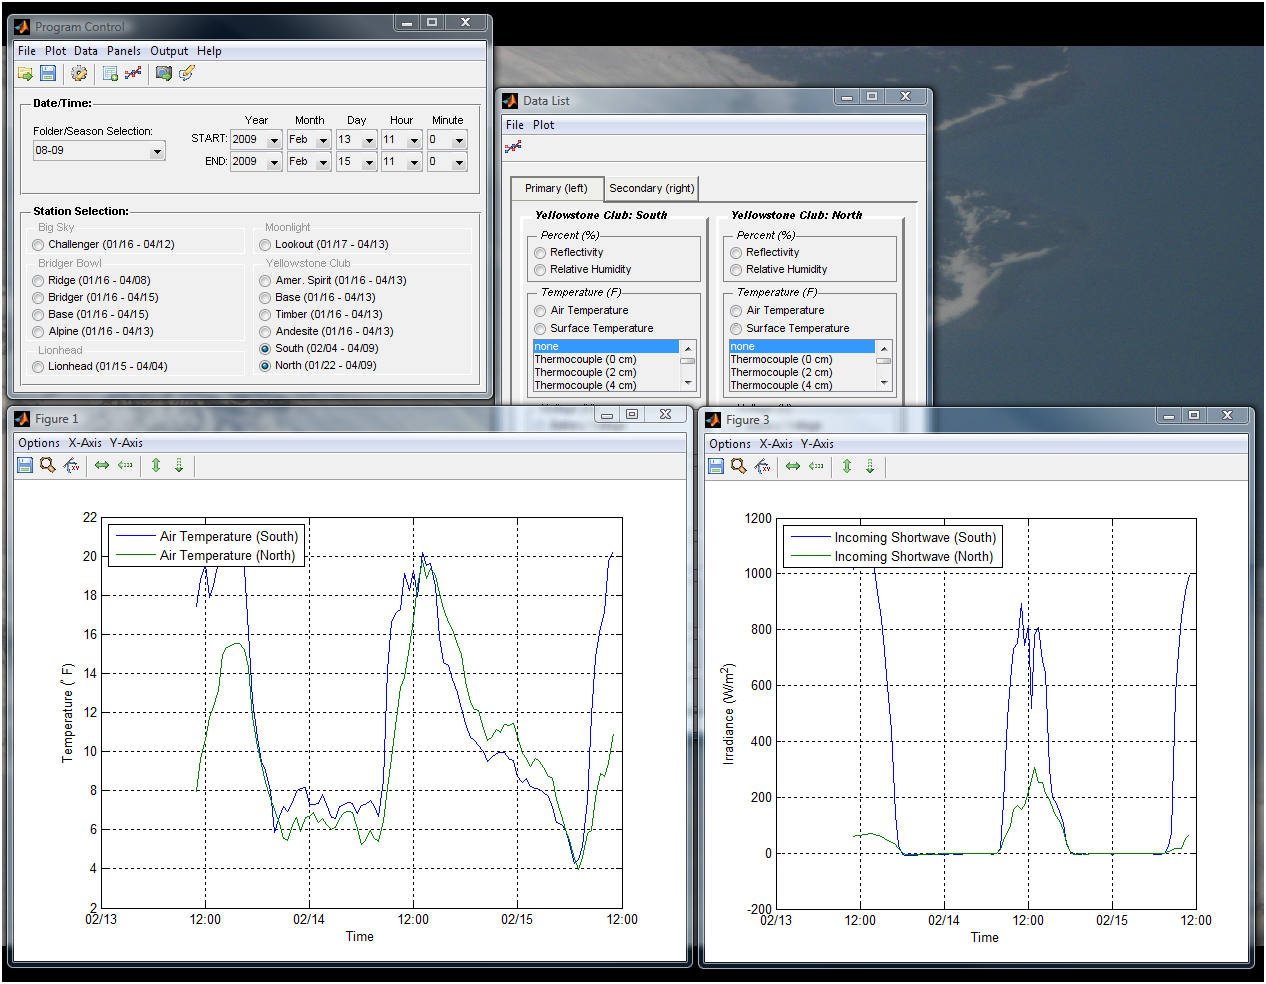
\includegraphics[width=\linewidth]{\YCfiles figures/wsexample.png}
	\caption{Example of a YCweather workspace.}
	\label{fig:wsexample}
\end{figure}

To create a workspace consider the following example:
\begin{enumerate}
	\item Begin by creating a graph of some kind, see Section \ref{sec:tutorial} for instruction on creating a graph.
	\item To create a second plot the Clear Figures preference must be turned off, see Section \ref{sec:pref} for details.
	\item Arrange the windows as desired.
	\item Save the workspace by selecting Save Workspace from the File menu in the Program Control window.  The default location is the \texttt{\bs saved} directory where YCweather was installed.  However, the workspace files (*.mat extension) may be saved in any location.
	\item The workspace is now saved.
\end{enumerate}

To load a workspace, simply select the Load Workspace option from the File menu and locate the desired workspace file in the dialog box that appears.  Once the workspace has been selected YCweather will provide a prompt, as in Figure \ref{fig:loadws}, that asks to use the current or stored time.  

\begin{figure}[ht!]\centering
	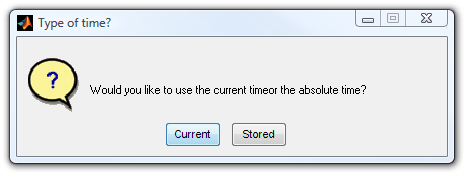
\includegraphics[width=0.55\linewidth]{\YCfiles figures/loadws.png}
	\caption{Prompt that appears by default when opening a workspace.}
	\label{fig:loadws}
\end{figure}

The ``current'' option, by default, recalls the workspace using the most recent 48 hrs of data that exists.  The stored time option uses the exact times set when the workspace was created.  These options exists so that the user can specify historical (``stored") workspaces of specific events or create workspaces (``current") of commonly used plots.  The YCweather preferences (Section \ref{sec:pref}) allow the number of hours to be changed as well as the prompt appearance to be changed.  For example, if a workspace is created that is solely intended for a specific event, then the prompting preference should be changed to ``Stored" so that when this workspace is recalled it simply opens.